\newpage
\subsection{Изготовление образцов продукции}
\label{bp:pattern}

% Вырезание образцов на плоттере. Оператору на плоттер приходит задание с чертежами в AUTOCADE по электронной почте. Заготовка попадает в план на гофроагрегат. Оператор плоттера смотрит план и ориентируется на графу «номенклатура» и «упаковка». Если они не заполнены, значит это заготовки на плоттер (ф 86). Далее он переносит чертеж из AUTOCADE в свою программу Impact (ф 89) и вырезает образцы. Далее, при необходимости склеивает их, упаковывает, прикрепляет ярлык (ф 88) и передает на склад готовой продукции, заполнив отчет (ф 90), который служит подтверждением передачи на склад. После заполняет отчет на сервере (ф 87) по которому ориентируются о выполнении заказчики образцов.




При необходимости выпуска образцов изделий для клиента (до 10 шт.) менеджер создает заявку в MS Excel на изготовление образцов (рис. \ref{pic:I.3}), которую передает в технологический отдел. 

При поступлении заказа на образцы мастер по ремонту и изготовлению оснастки разрабатывает чертеж изделия и затем  вырезает необходимое количество образцов на плоттере (рис. \ref{pic:II плоттер}).

На ПРЕДПРИЯТИИ для изготовления образцов предусмотрен плановый выпуск листового картона разных марок (рис. \ref{pic:II заготовки для образцов}).   
%Конструктор на основании полученной служебной записки и макета вырезает на плоттере образец. 

На плоттере можно вырезать партию до 50 штук (по согласованию с директором филиала). При необходимости большего объема менеджер создает  заявку для производства заготовок на гофроагрегате под образцы.
%Менеджер самостоятельно опрашивает конструктора о готовности образцов.
После изготовления требуемого количества образцов мастер по ремонту и изготовлению оснастки фиксирует в MS Excel  факт выполнения заявки. 

Образцы производятся за счет Предприятия.

%Менеджер при обращении покупателя создаёт служебную записку на изготовление образцов (форма \ref{pic:pic_d1}). Образцы продукции изготавливает вручную специалист в конструкторском отделе.  %Максимальное количество образцов изготавливается до 10 штук. Менеджер оставляет копию служебной записки у себя для контроля производства образцов. 
%Журнал учёта образцов не ведётся. 
%Вырезается на один образец больше. Дополнительный образец хранится в отделе штампов до принятия окончательного решения заказчиком. Готовые образцы передаются менеджерам с ярлыком. 
\newpage
\begin{figure}
\begin{center}
 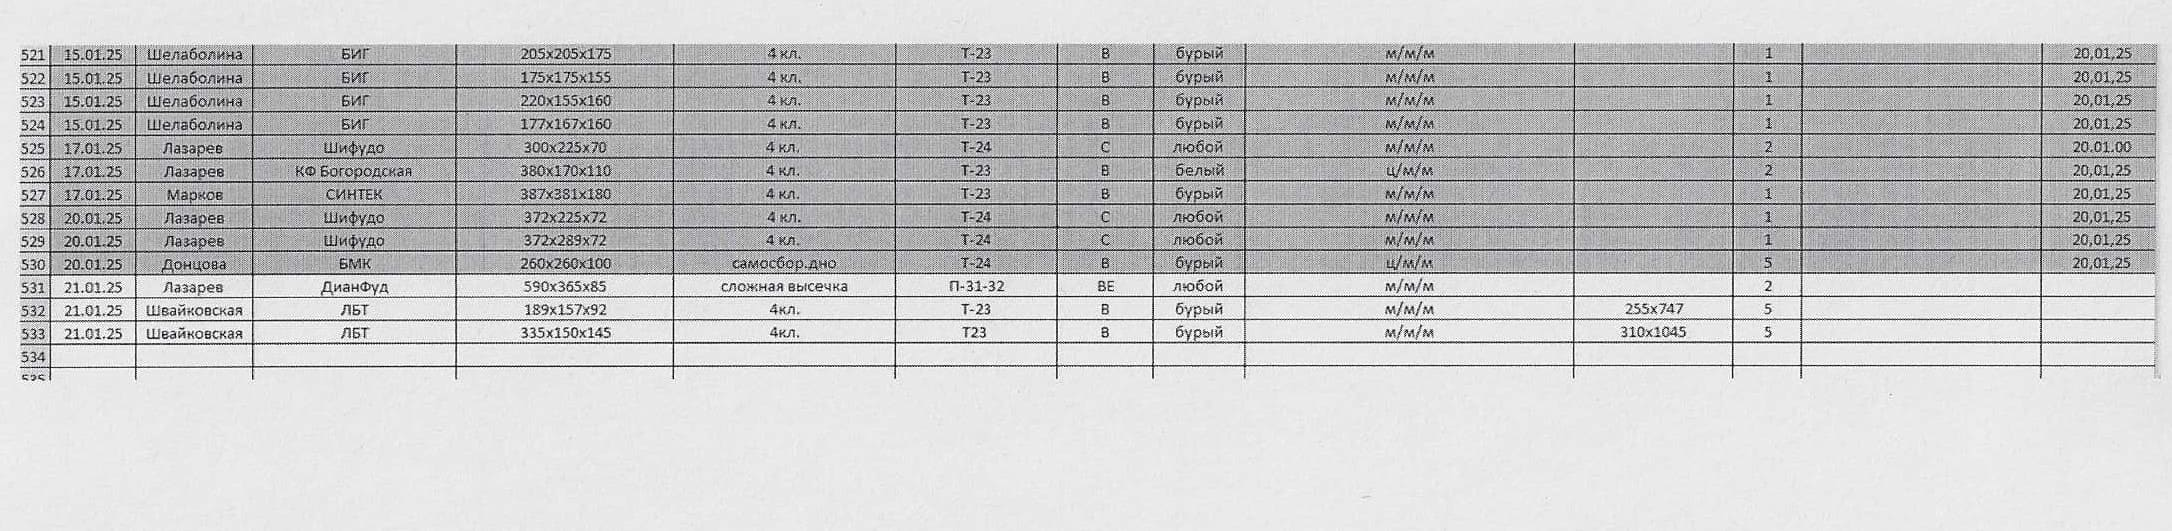
\includegraphics[height=0.16\textheight, keepaspectratio]{Pics/I.3.jpg}
\end{center}
 \caption{Заявки на изготовление образцов}
 \label{pic:I.3}
\end{figure}

\begin{figure}
\begin{center}
 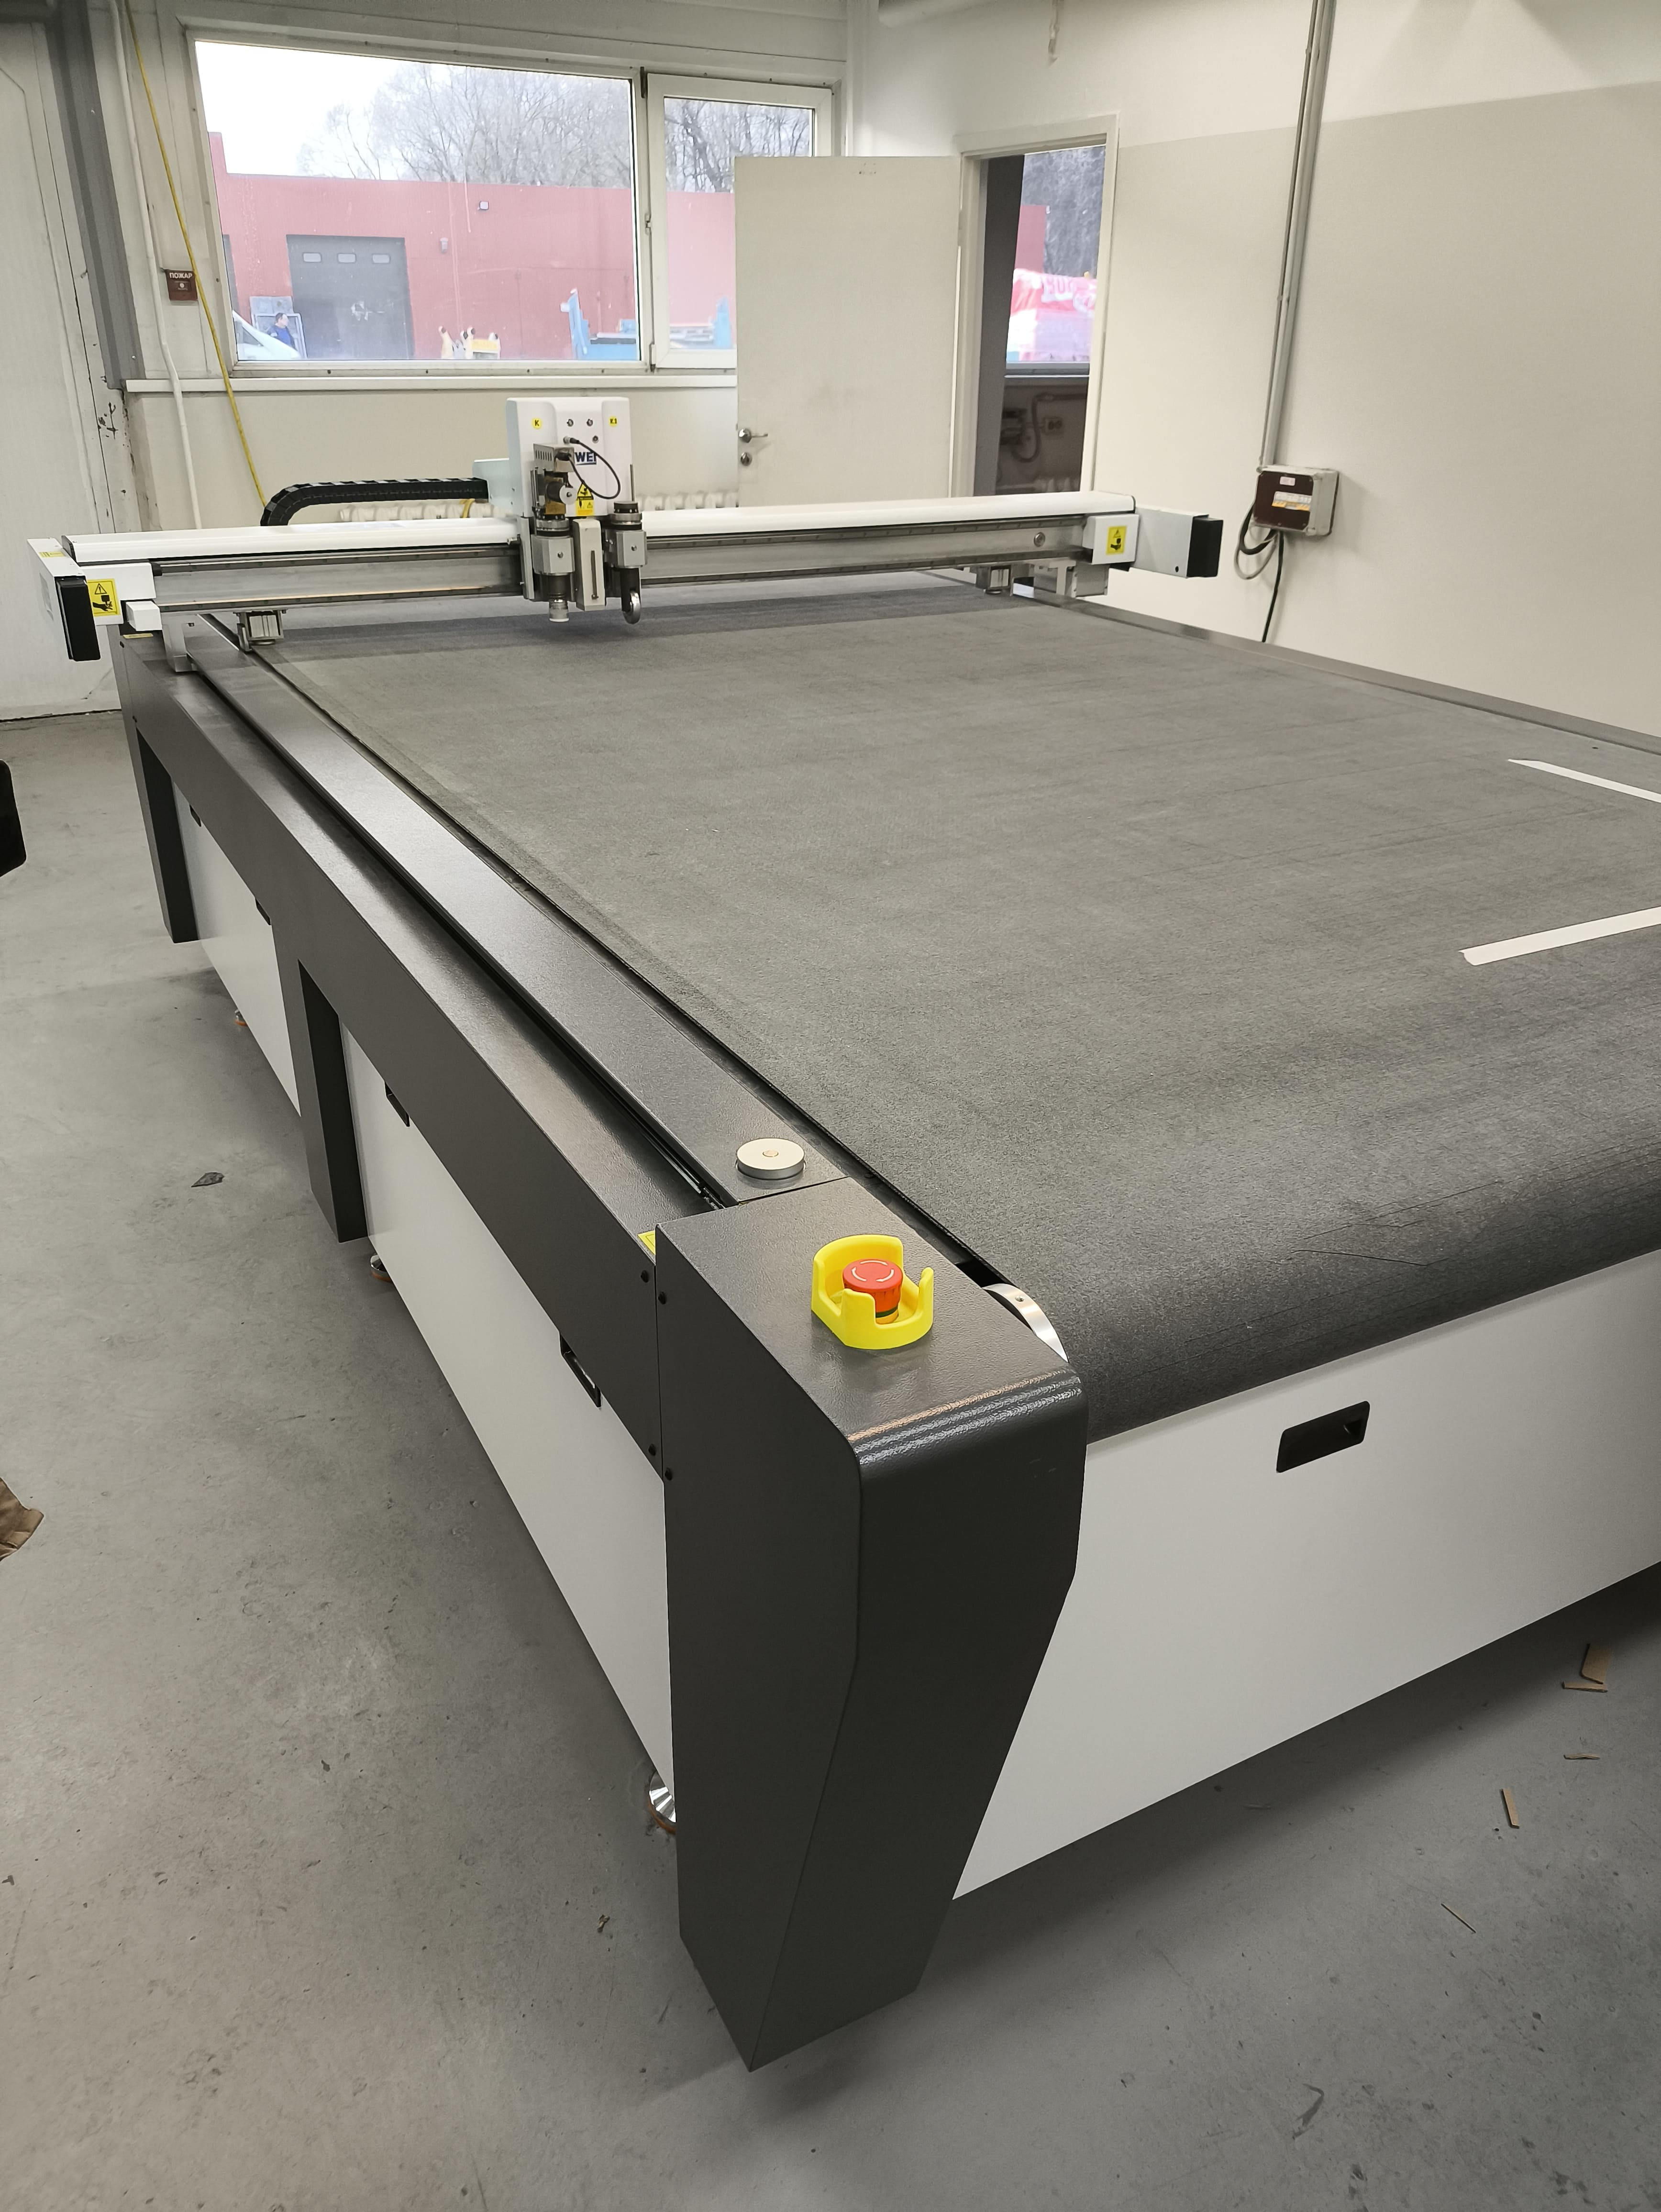
\includegraphics[height=0.6\textheight, keepaspectratio]{Pics/II плоттер.jpg}
\end{center}
 \caption{Плоттер}
 \label{pic:II плоттер}
\end{figure}

\begin{figure}
\begin{center}
 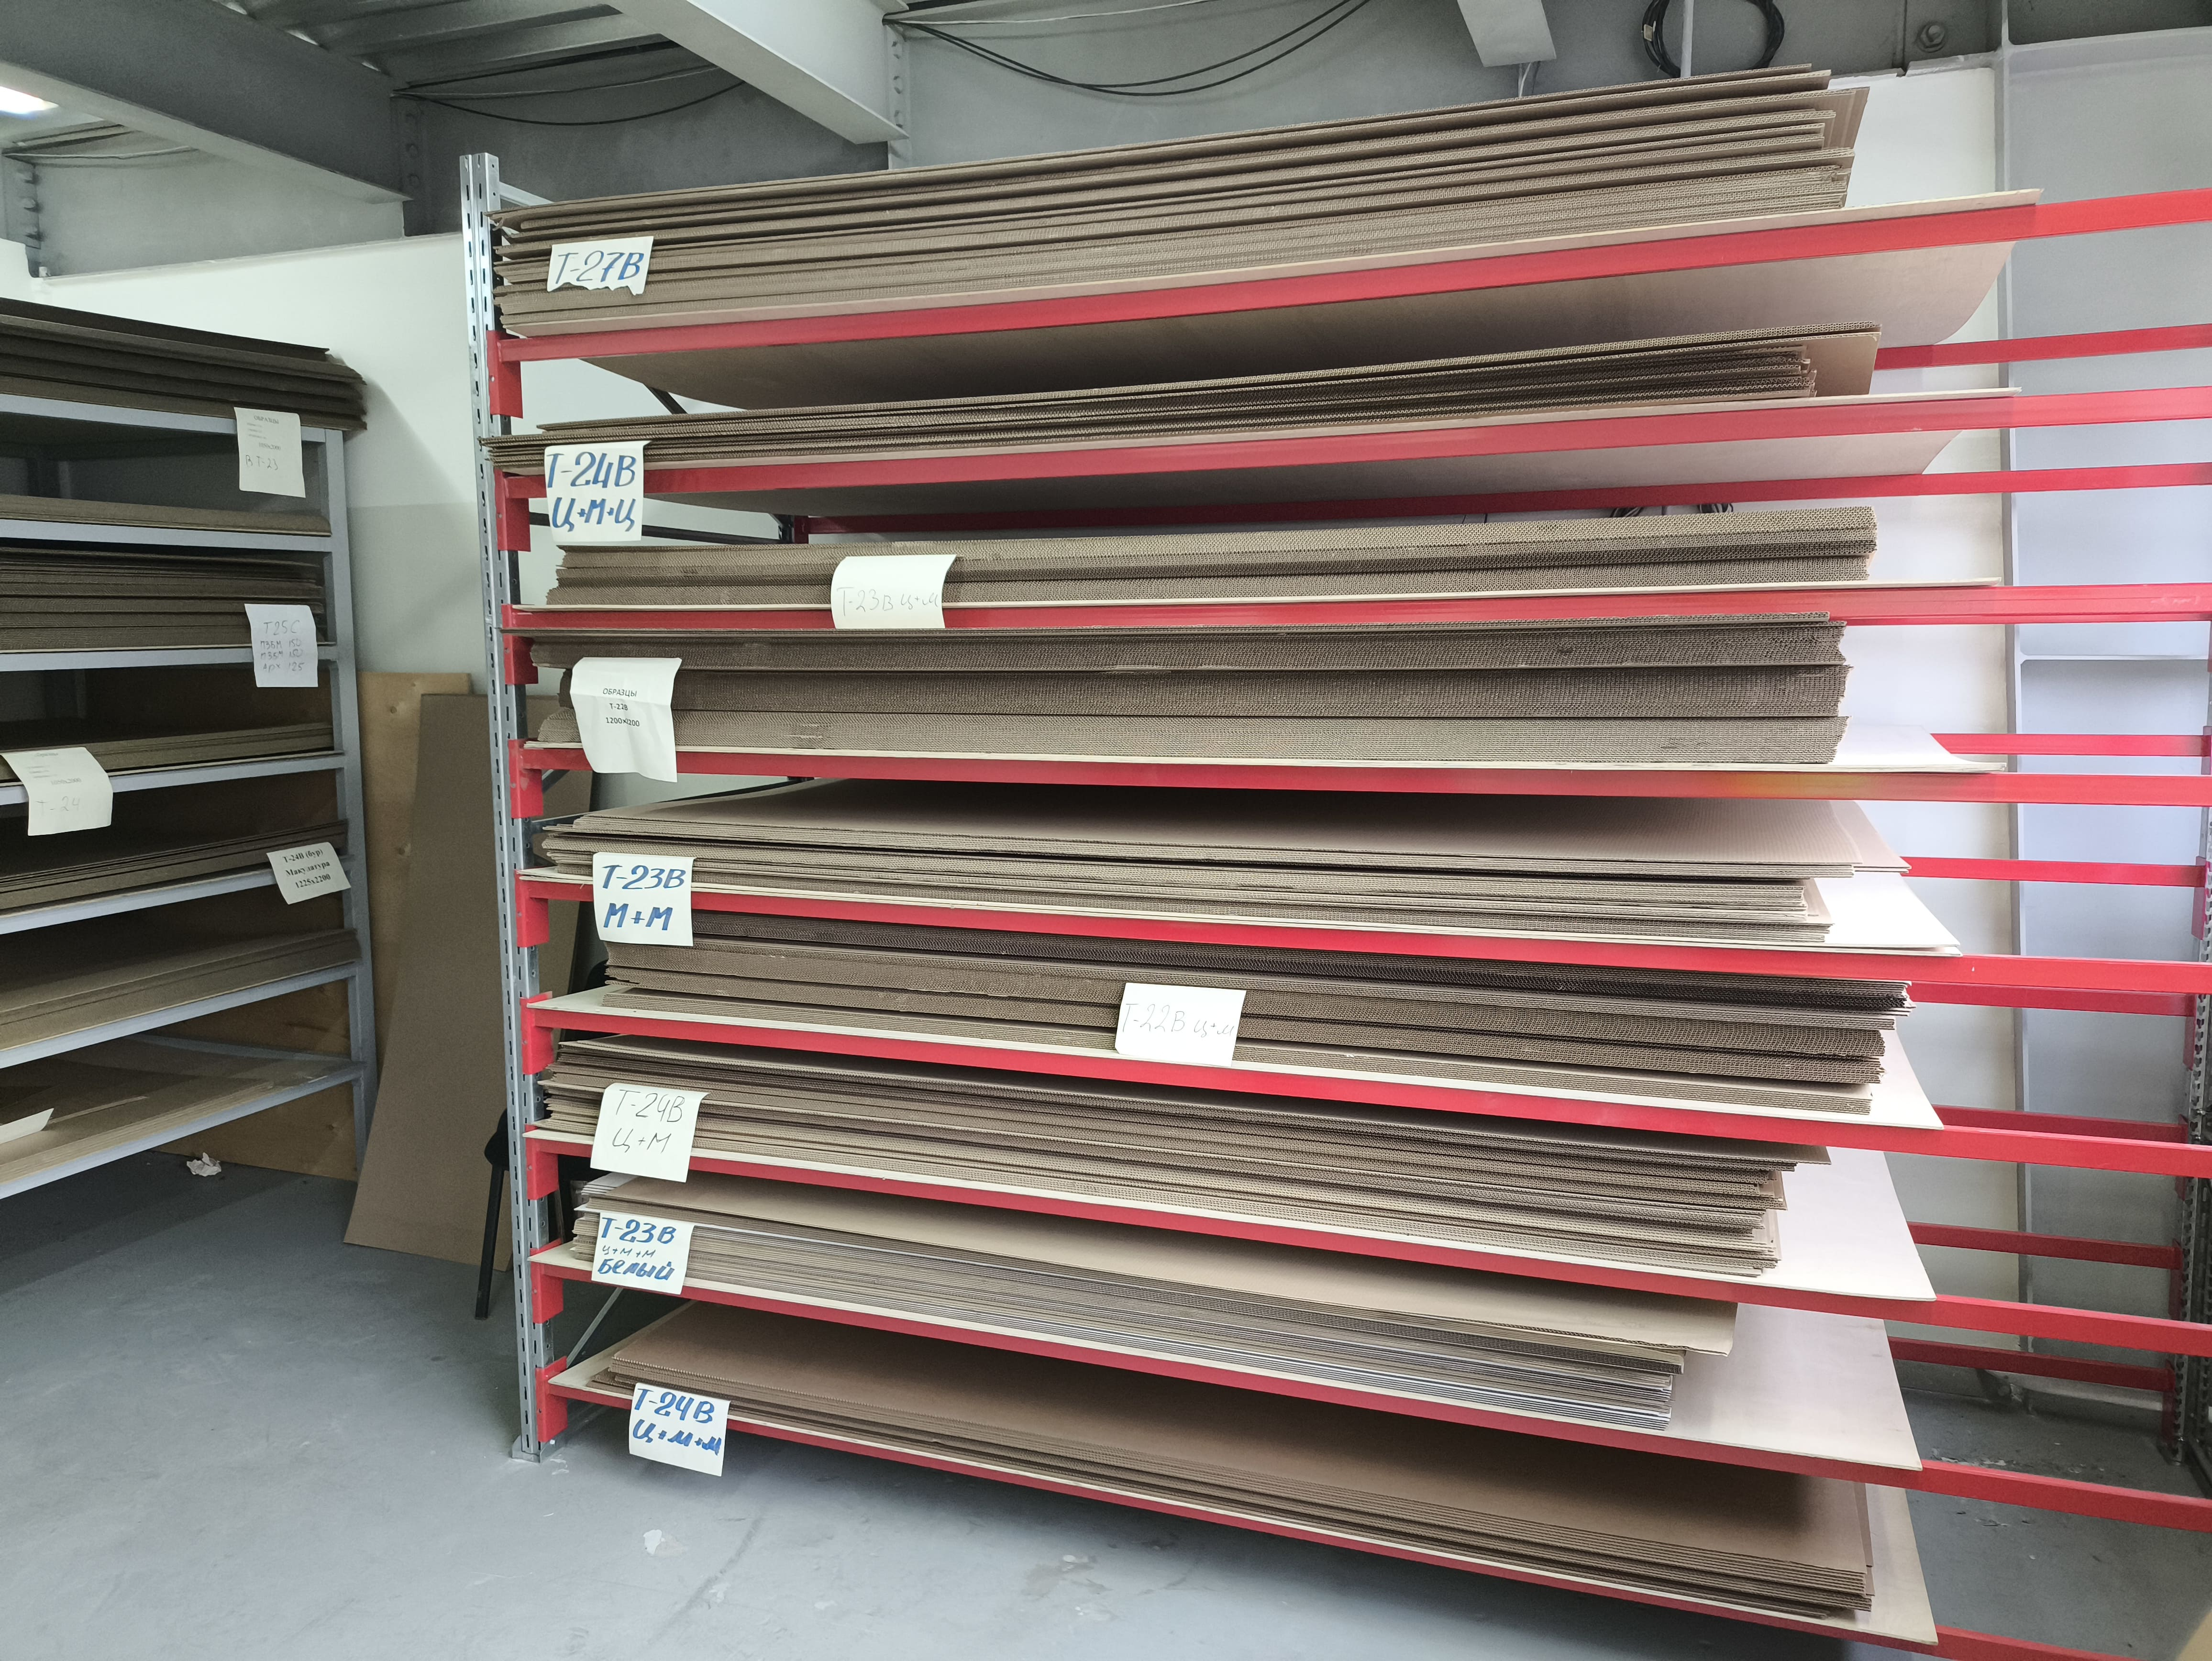
\includegraphics[height=0.5\textheight, keepaspectratio]{Pics/II заготовки для образцов.jpg}
\end{center}
 \caption{Заготовки для изготовления образцов изделий}
 \label{pic:II заготовки для образцов}
\end{figure}
\clearpage
\ifx \notincludehead\undefined
\normalsize
\end{document}
\fi